\chapter{Erstes Kapitel}
\section{Erster Abschnitt}

Hier beginnt der erste Satz, der dann gleich mit einem Bild weitergeführt wird
\begin{figure}[htbp]
\centering
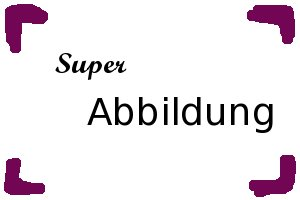
\includegraphics[width=0.7\textwidth]{abbildungsdatei} % Datei in "bilder/" bei LaTeX: eps, bei PDFLaTeX: jpg (o.ä.) 
\caption{Titel der Abbildung} 
\label{fig:bild1}
\end{figure}

In der Abbildung~\ref{fig:bild1}\footnote{vgl. Zitat A\cite{referenzA}} % referenzA muss im Verzeichnis literatur in der Datei bib.bib enthalten sein
ist zu sehen, dass ...

% Neue Seite
\newpage

\section{Und nächster Abschnitt etwas länger als vorher es war}
Eine neue Seite, um auchmal die Kopfzeile zu sehen, da sie auf Seiten mit Kapitelanfang nicht erscheinen. Eine Abkürzung ist z.B. etc.\abbrev{etc.}{et cetera}, welche im 
Abkürzungsverzeichnis erklärt wird. 
